\section{Développer une expression littérale}

\subsection{La distributivité simple}

\begin{propriete}
Soient $k$, $a$ et $b$ trois nombres relatifs. Pour \MotDefinition{développer une expression}{}, on distribue un facteur à tous les termes entre parenthèses :

\begin{align*}
    \boldsymbol{k \times} (a + b) &= \boldsymbol{k \times} a + \boldsymbol{k \times} b\\
    \boldsymbol{k \times} (a - b) &= \boldsymbol{k \times} a - \boldsymbol{k \times} b\\
\end{align*}

%\begin{center}
%    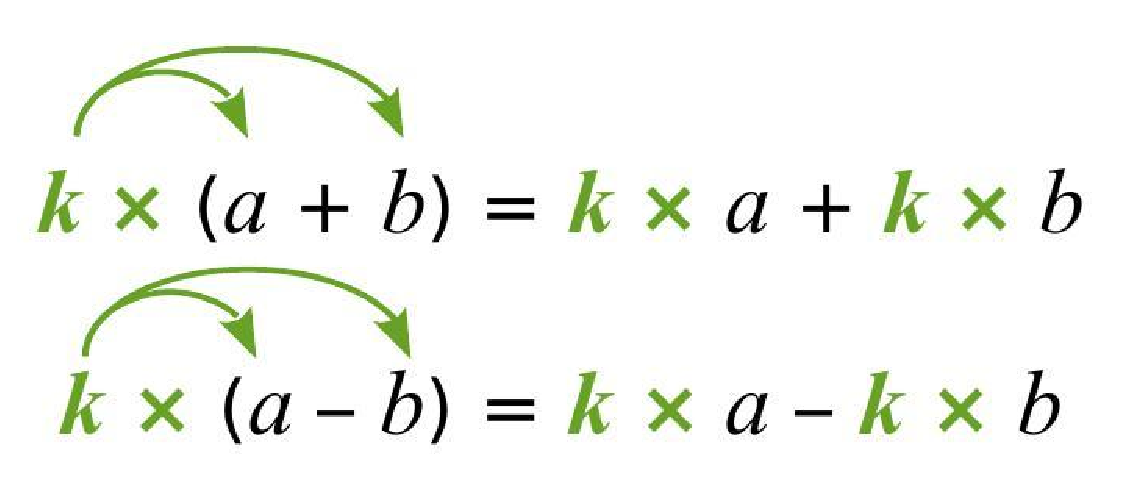
\includegraphics[width=.35\linewidth]{DiC01}
%\end{center}
\end{propriete} 


\begin{exemple*1}

Développe l'expression suivante : $C = - 3,5(x - 2)$.

\correction

\begin{tabular}{lcl}
$C = \boldsymbol{- 3,5 \times} (x - 2)$ & $\longrightarrow$ & On replace le signe $\boldsymbol{\times}$ dans l'expression. \\
$C = \boldsymbol{(- 3,5)} \times x + \boldsymbol{(- 3,5)} \times (- 2)$ & $\longrightarrow$ & On distribue le facteur $-3,5$ aux termes $x$ et $-2$. \\
$C = - 3,5x + 7$ & $\longrightarrow$ & On calcule et on simplifie l'expression. \\
\end{tabular}
\end{exemple*1}




\subsection{Cas particulier : \MotDefinition{distribuer un signe $-$}{}}

\begin{propriete}
Lorsqu'une parenthèse est précédée d'une signe $-$, c'est comme si toute la parenthèse était multipliée par $-1$. Le moins se distribue donc comme un nombre, en utilisant la règle du produit des signes :
\begin{align*}
    \boldsymbol{-1 \times} (a + b) &= \boldsymbol{-1 \times} a + \boldsymbol{( -1 ) \times} b = - a + (-b) = - a - b \\
    \boldsymbol{-1 \times} (a - b) &= \boldsymbol{-1 \times} a - \boldsymbol{( -1 ) \times} b = - a - (-b) = - a + b \\
\end{align*}

%\begin{center}
%    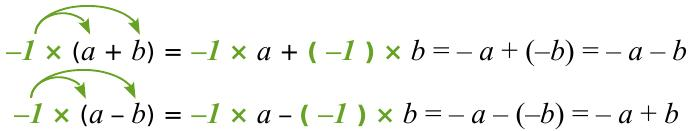
\includegraphics[width=.65\linewidth]{DiC02}
%\end{center}
\end{propriete}

\begin{exemple*1}

Développe l'expression suivante : $A = - (x - 2) + (- 2x + 3) - (-1 - 2x)$.

\correction

\begin{tabular}{lcl}
$A = - (x - 2) + (- 2x + 3) - (-1 - 2x)$ & & \\
$A =  - x + 2 + (- 2x + 3) +1 + 2x$ & $\longrightarrow$ & On distribue le signe $-$ de la 1\up{ère} et de la 3\up{e} parenthèse. \\
$A = - x + 2 - 2x + 3 +1 + 2x$ & $\longrightarrow$ & On peut enlever la parenthèse précédée d'un $+$. \\
$A = - 3x + 6$ & $\longrightarrow$ & On calcule et on simplifie l'expression. \\
\end{tabular}
\end{exemple*1}





\subsection{La \MotDefinition{double distributivité}{}}


\begin{propriete}
Pour tous nombres relatifs $a$, $b$, $c$ et $d$ :

\begin{minipage}[c]{.6\linewidth}
    \centering
    $(\boldsymbol{a} + \boldsymbol{b})(c + d) = \boldsymbol{a}c + \boldsymbol{a}d + \boldsymbol{b}c + \boldsymbol{b}d$
    %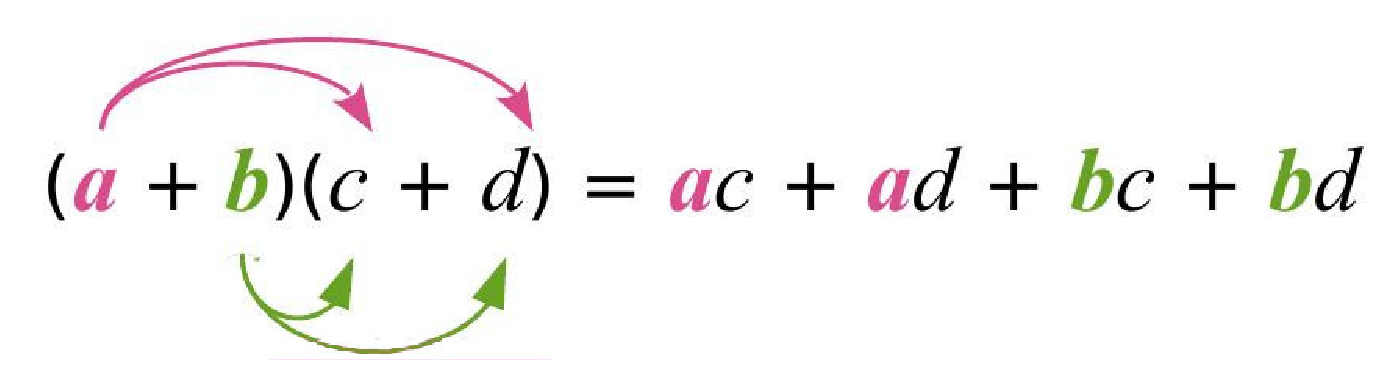
\includegraphics[width=\linewidth]{DiC03}
\end{minipage}%
\hfill%
\begin{minipage}[c]{.38\linewidth}
    \centering
    
\includegraphics[width=.7\linewidth]{DiC04}
\end{minipage}
\end{propriete} 

\begin{exemple*1}

Développe et simplifie l'expression suivante : $D = (3x + 1)(y - 4)$.

\correction

\begin{tabular}{lcl}
$D = (3x + 1)(y + (- 4))$ & $\longrightarrow$ & On transforme la soustraction. \\
$D = \boldsymbol{3x \times} y + \boldsymbol{3x \times} (- 4) + \boldsymbol{1 \times} y + \boldsymbol{1 \times} (- 4)$ & $\longrightarrow$ & On applique la double distributivité. \\
$D = 3xy - 12x + y - 4$ & $\longrightarrow$ & On calcule les produits et on simplifie. \\
\end{tabular}
\end{exemple*1}





